\documentclass[final,hyperref={pdfpagelabels=false}]{beamer}

\mode<presentation>
  {
  %  \usetheme{Berlin}
  \usetheme{uclposter}
  \usecolortheme{ucl}

  \setbeamercolor{block body}{bg=white,fg=black}


  }
  \usepackage{times}
  \usepackage{amsmath,amsthm, amssymb, latexsym}
  \boldmath
  \usepackage[english]{babel}
  \usepackage[latin1]{inputenc}
  \usepackage[orientation=landscape,size=a0,scale=1.4,debug]{beamerposter}

  %%%%%%%%%%%%%%%%%%%%%%%%%%%%%%%%%%%%%%%%%%%%%%%%%%%%%%%%%%%%%%%%%%%%%%%%%%%%%%%%%5
  \graphicspath{{figures/}}
  \title[GVHD]{Computational analysis of gene expression datasets to unravel the basis of graft versus host disease}
  \author[Winship \& Plagnol]{Claire Winship, many others, Ron Chakraverty, Vincent Plagnol}
  \institute[UGI]{UCL Genetics Institute}
  \date{\today}

  %%%%%%%%%%%%%%%%%%%%%%%%%%%%%%%%%%%%%%%%%%%%%%%%%%%%%%%%%%%%%%%%%%%%%%%%%%%%%%%%%5
  \begin{document}

  \begin{frame}{} 

  \begin{beamercolorbox}{}
    \maketitle
  \end{beamercolorbox}


    \vfill
    \begin{columns}[t]

      \begin{column}{.25\linewidth}
        \begin{block}{Graft versus host disease}
     \begin{itemize}
          \item In malignant pathologies the donor immune system recognises tumour cells as foreign and eradicates them via immunological mechanisms which together are known as the graft vs tumour (GVT) effect
          \item Donor immune cells may also attack normal host tissue resulting in acute graft vs host disease (GVHD)
          \item The skin, liver and gastrointestinal tract are the most common tissues to be damaged in GVHD
          \item GVHD remains one of the most common post-transplant complications and represents a major barrier to the successful application of allo-HSCT
	  \item A major risk factor involved in GVHD pathology is the use of HLA-mismatched, non related donors
          \item Acute GVHD involves alloreactive donor T-cell mediated cytotoxic response to the tissues of the recipient
          \item Tissue damage caused by cytotoxic T cells leads to recruitment of other effector cells including natural killer cells which further increases tissue injury and results in self perpetuating GVHD
          \item Mice represents the primary model animal for pre-clinical studies of GVHD
          \item Mouse models of acute GVHD usually involve a bone marrow transplant (BMT) which is supplemented with varying numbers/types of donor lymphocites into irradiated allogenic recipients who differ from donors in their MHC class 1 and/or class 2 molecules or in minor histocompatibility antigens
          \end{itemize} 
        \end{block}


        \begin{block}{The ImmGene project}
          \begin{itemize}
          \item some items
          \item some items
          \item some items
          \item some items
          \end{itemize}
        \end{block}

      \end{column}


      \begin{column}{.24\linewidth}
        \begin{block}{T-cell expression in multiple minor histocompatibility antigen-mismatched BMT model}
	  {\bf Objective:} In a polyclonal model, evaluate the differences in gene expression of effector T cells found in the lymphoid organs or in the peripheral tissues.

	  \begin{minipage}{0.45\textwidth}
	    \includegraphics[width=13cm]{/cluster/project8/vyp/Winship_GVHD/claire/results/mhc1_ko/figs/PCA_prettier.pdf}
	  \end{minipage}	  
	  \begin{minipage}{0.45\textwidth}
	    \includegraphics[width=13cm]{/cluster/project8/vyp/Winship_GVHD/claire/results/mhc1_ko/figs/PCA_prettier_outlier_removed.pdf}
	  \end{minipage}	  
	  {\small
          \begin{itemize}
          \item PCA analysis of all samples reveals presence of outlier in the D7 dataset ($TM008_ko4$)
          \item some items
          \item some items
          \end{itemize} }
	  \begin{minipage}{0.45\textwidth}
            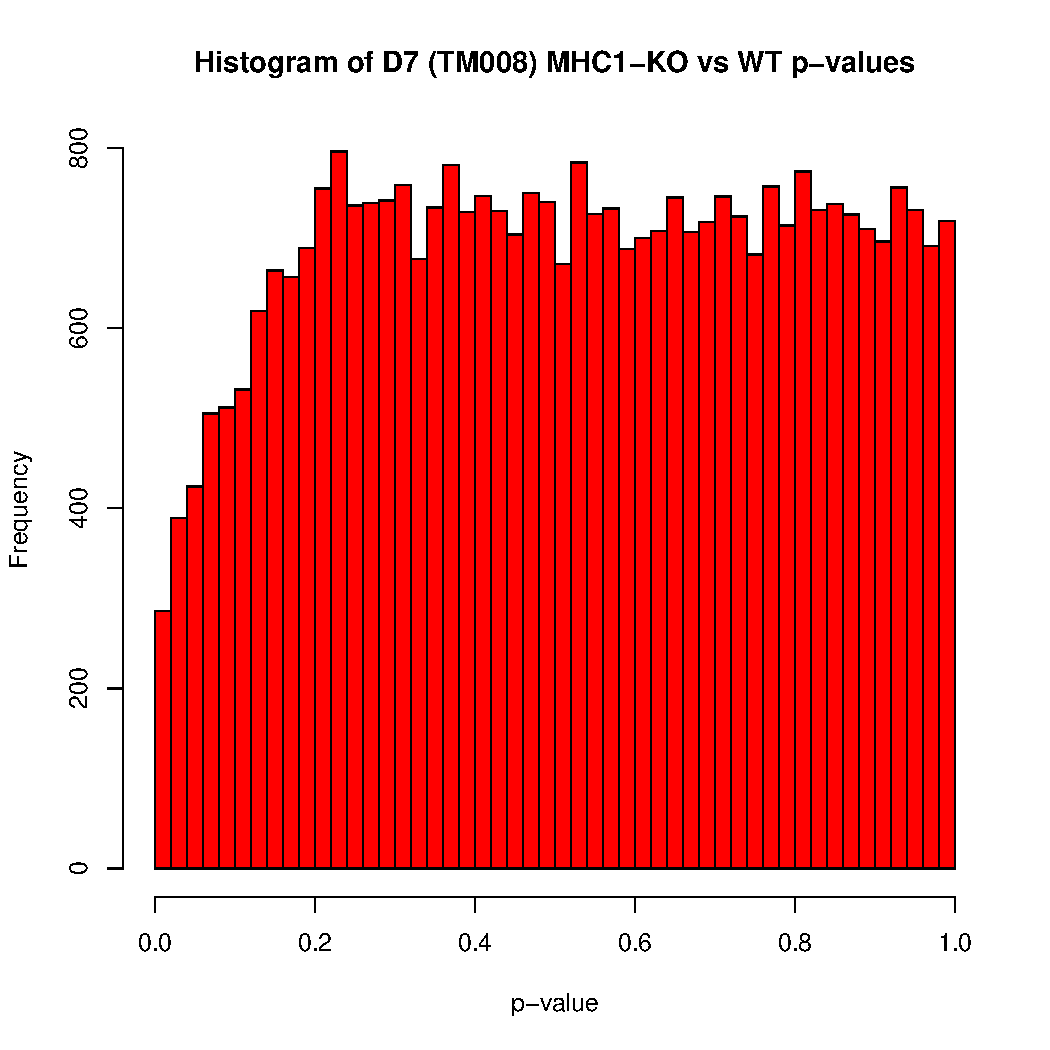
\includegraphics[width=13cm]{/cluster/project8/vyp/Winship_GVHD/claire/results/mhc1_ko/figs/D7_histogram.pdf}
          \end{minipage}
	  \begin{minipage}{0.45\textwidth}
            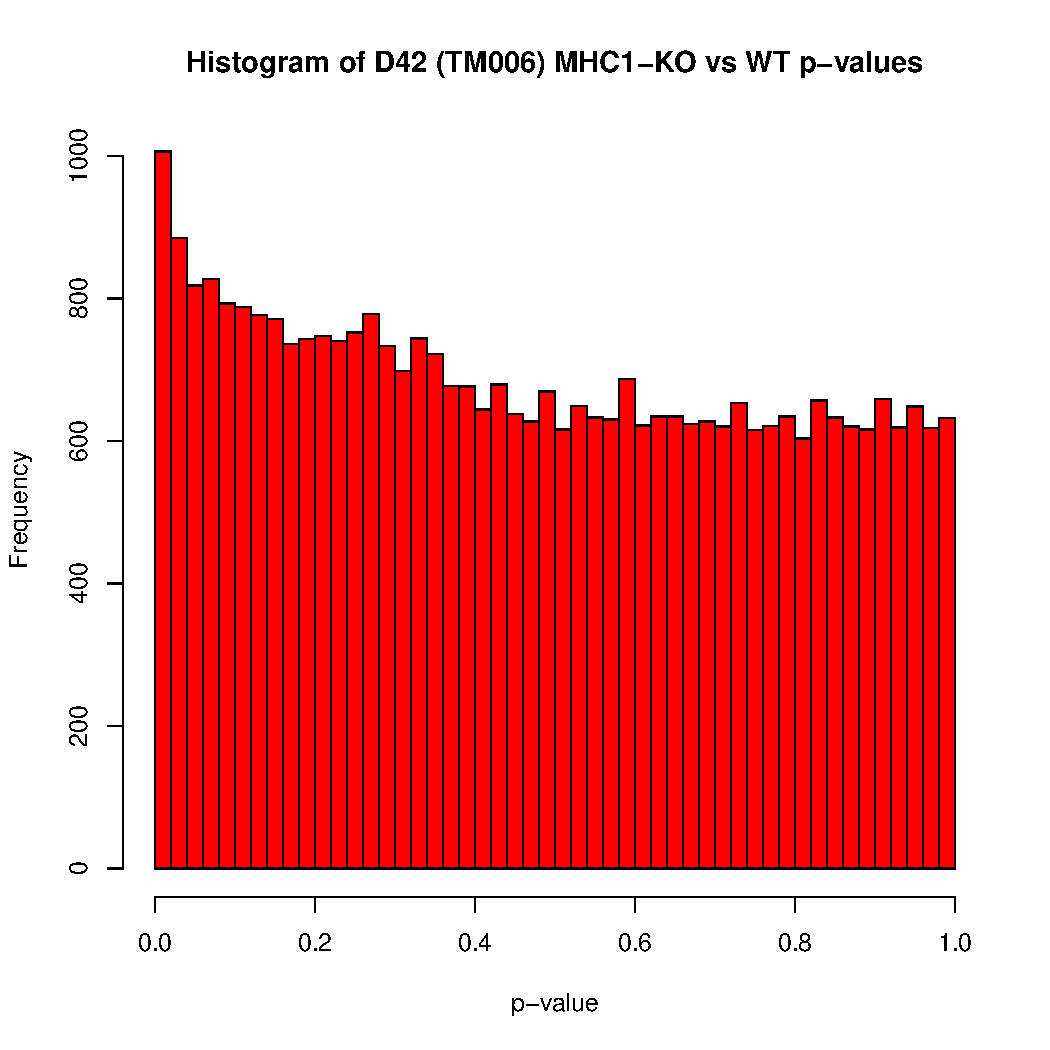
\includegraphics[width=13cm]{/cluster/project8/vyp/Winship_GVHD/claire/results/mhc1_ko/figs/D42_histogram.pdf}
          \end{minipage}
{\small
	  \begin{itemize}
	    \item some items
	    \item some items
	    \end{itemize} }
          \begin{minipage}{0.45\textwidth}
            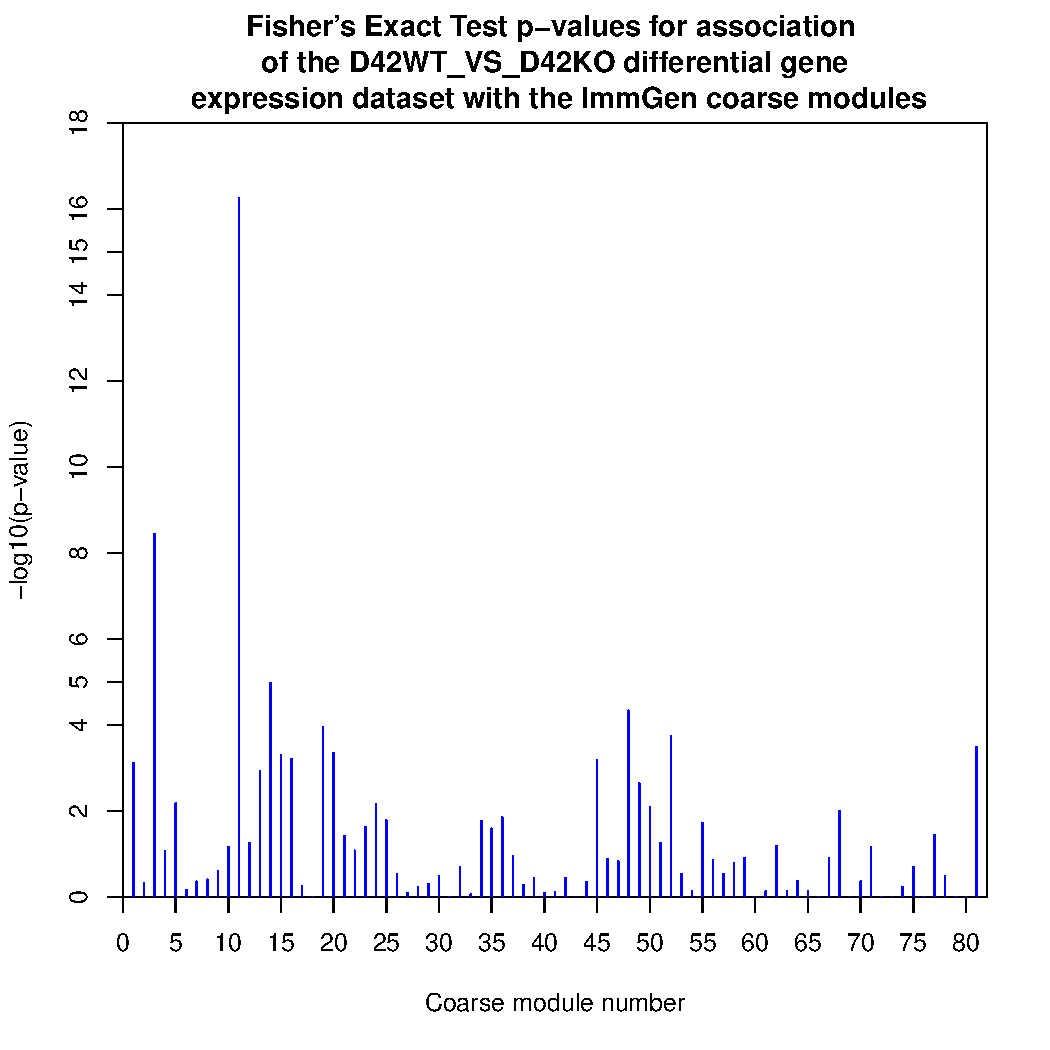
\includegraphics[width=13cm]{/cluster/project8/vyp/Winship_GVHD/claire/results/mhc1_ko/figs/D42WT_VS_D42KO_coarse_module_association_graph.pdf}
          \end{minipage}
          \begin{minipage}{0.45\textwidth}
            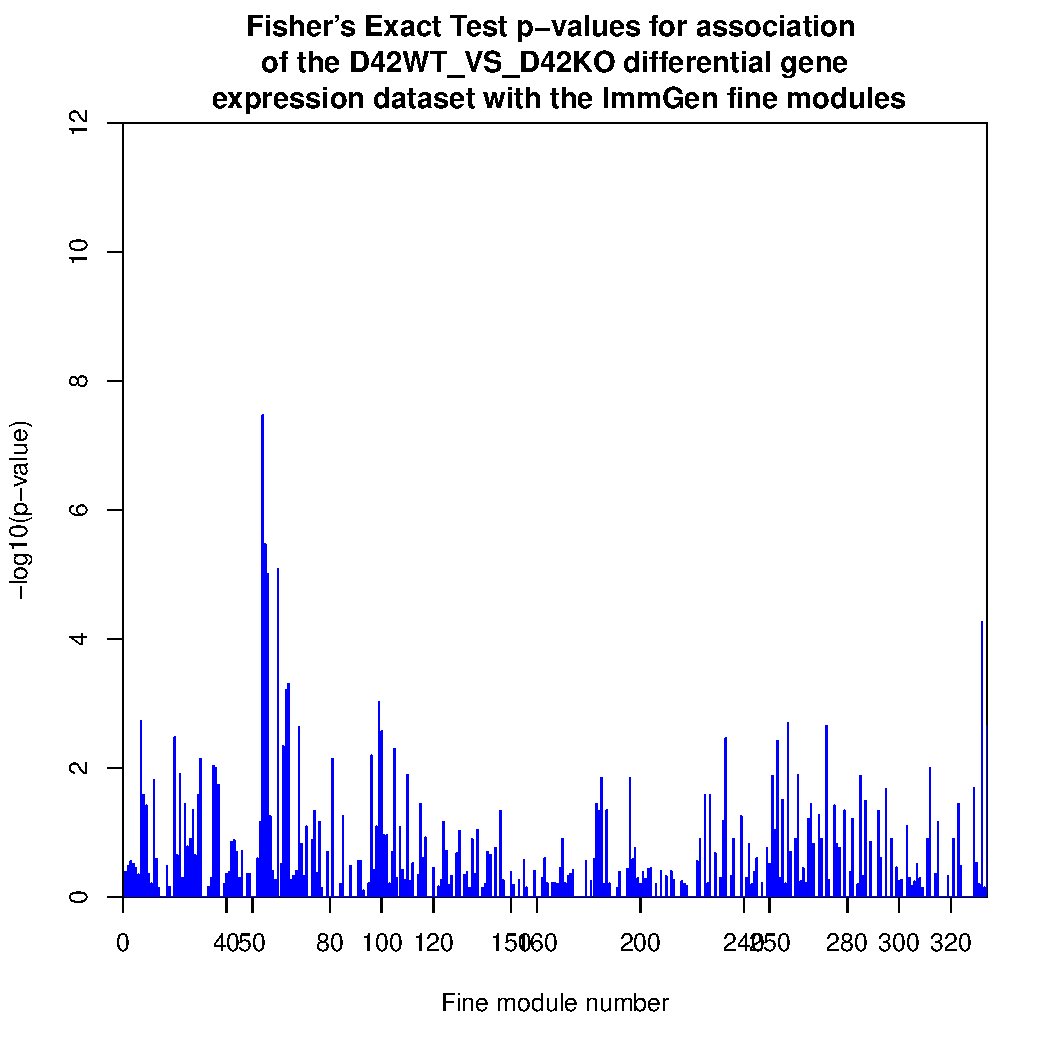
\includegraphics[width=13cm]{/cluster/project8/vyp/Winship_GVHD/claire/results/mhc1_ko/figs/D42WT_VS_D42KO_fine_module_association_graph.pdf}
          \end{minipage}
	  \begin{center}
	{\small    \begin{tabular}{ |c|c|c| } 
	      \hline
	      gene name & fold change & pvalue \\
	      \hline
	      Ptbp2 & 0.8575669378 & 0.0002380649 \\
	      Trappc1 & -0.8105321657 & 0.0011522667 \\
	      Mrpl32 & -0.9482075354 & 0.0015174569 \\
	      Ctso & 0.6665616898 & 0.0015502065 \\
	      Cib1 & -0.5435813927 & 0.0022304297 \\
	      Chordc1  & -1.1641319443 & 0.0033252187 \\
	      Actr6 & -0.7619741241 & 0.0034636625 \\
	      Pcgf5 & -0.6144202783 & 0.0035618031 \\
	      Llph & -0.797961394 & 0.0047160713 \\
	      1810037I17Rik & -0.6327137658 & 0.0053622021 \\
	      Cd46 & 1.2478436705 & 0.0077584292 \\
	      Zfp455 & -1.3221395229 & 0.0083646381 \\
	      \hline
	    \end{tabular} }
	  \end{center}
        \end{block}
      \end{column}
      \begin{column}{.25\linewidth}
        \begin{block}{T-cell expression: Single minor histocompatibility antigen-mismatched BMT model}
	  {\bf Objective:} In a monoclonal model, evaluate the effect of depleting Langerhans cells on the gene expression of effector T cells found in the lymph nodes and in the skin.
	  \begin{center}
	   \includegraphics[width=15cm]{/cluster/project8/vyp/Winship_GVHD/claire/results/epi_dermis_PLN/figs/PCA_prettier.pdf}
            \end{center}
{\small          \begin{itemize}
          \item some items
          \item some items
          \item some items
          \item some items
          \end{itemize}}
	  \begin{minipage}{0.45\textwidth}
            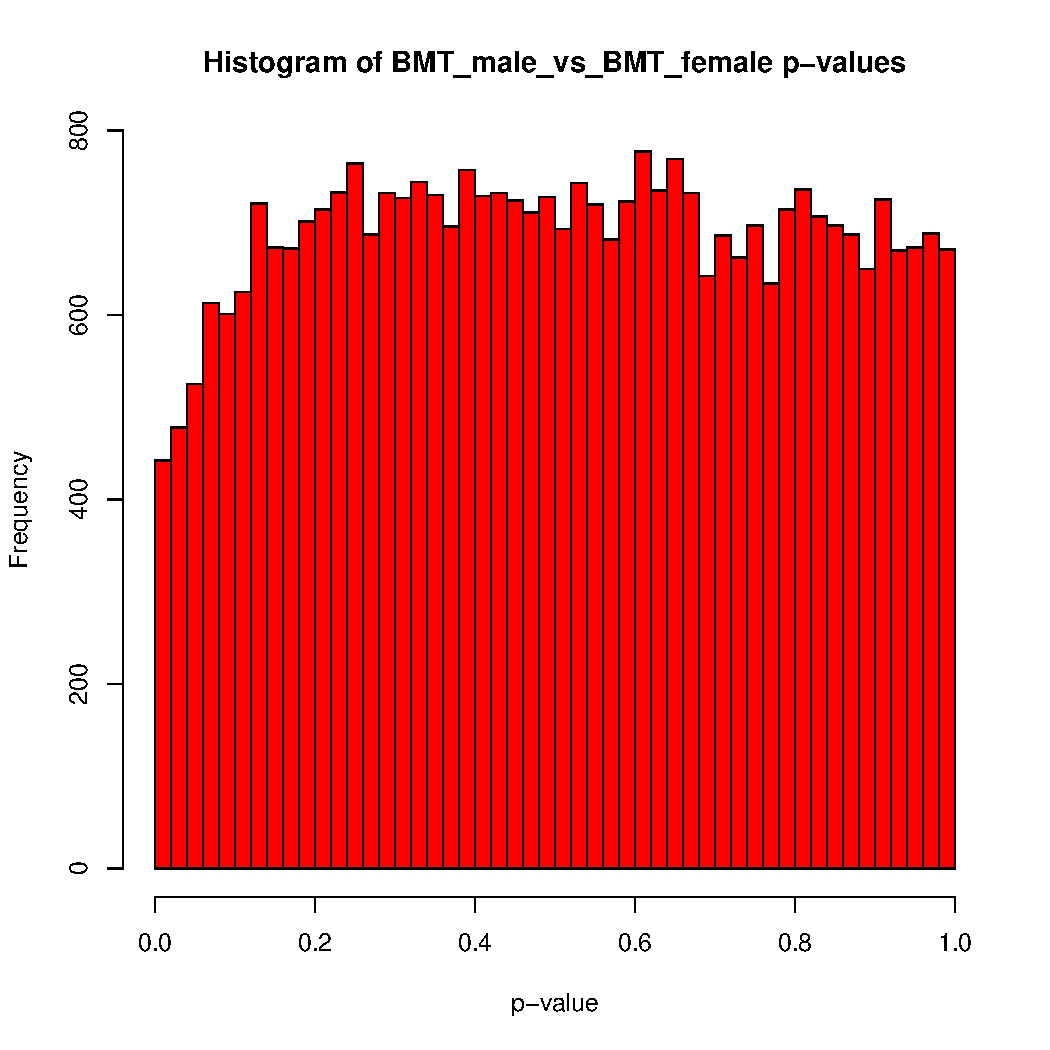
\includegraphics[width=13cm]{/cluster/project8/vyp/Winship_GVHD/claire/results/syn_allo_bmt/figs/BMT_male_vs_BMT_female_histogram.pdf}
          \end{minipage}
          \begin{minipage}{0.45\textwidth}
            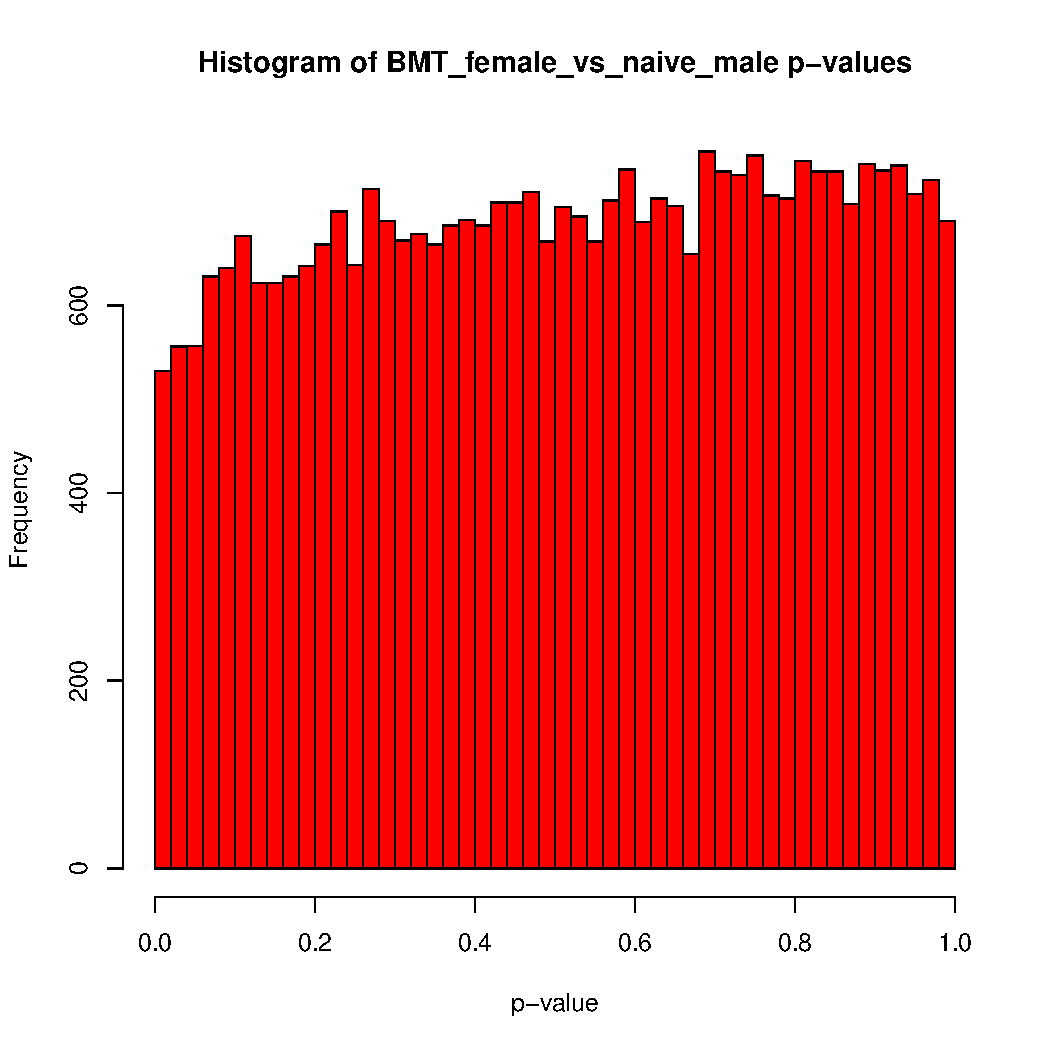
\includegraphics[width=13cm]{/cluster/project8/vyp/Winship_GVHD/claire/results/syn_allo_bmt/figs/BMT_female_vs_naive_male_histogram.pdf}
          \end{minipage}
{\small	  \begin{itemize}
	    \item Histogram of BMT male vs naive male p-values appears to show a more consistent distribution with the null hypothesis 
	    \item some items
	   \end{itemize}}
	  \begin{minipage}{0.45\textwidth}
            \includegraphics[width=13cm]{/cluster/project8/vyp/Winship_GVHD/claire/results/syn_allo_bmt/figs/BMT_male_vs_BMT_female_coarse_module_association_graph.pdf}
          \end{minipage}
          \begin{minipage}{0.45\textwidth}
            \includegraphics[width=13cm]{/cluster/project8/vyp/Winship_GVHD/claire/results/syn_allo_bmt/figs/BMT_female_vs_naive_male_coarse_module_association_graph.pdf}
          \end{minipage}
	  \begin{minipage}{0.45\textwidth}
            \includegraphics[width=13cm]{/cluster/project8/vyp/Winship_GVHD/claire/results/syn_allo_bmt/figs/BMT_female_vs_naive_male_fine_module_association_graph.pdf}
          \end{minipage}
          \begin{minipage}{0.45\textwidth}
            \includegraphics[width=13cm]{/cluster/project8/vyp/Winship_GVHD/claire/results/syn_allo_bmt/figs/BMT_male_vs_naive_male_coarse_module_association_graph.pdf}
          \end{minipage}
	  \begin{minipage}{0.45\textwidth}
            \includegraphics[width=13cm]{/cluster/project8/vyp/Winship_GVHD/claire/results/syn_allo_bmt/figs/BMT_male_vs_naive_male_fine_module_association_graph.pdf}
          \end{minipage}
        \end{block}
      \end{column}


      \begin{column}{.25\linewidth}
        \begin{block}{Langerhans cell expression}
	  {\bf Objective:} Evaluate the differences in gene expression of Langerhans cells in the setting of an allogeneic BMT or a syngeneic BMT.
           \begin{center}
           \includegraphics[width=15cm]{/cluster/project8/vyp/Winship_GVHD/claire/results/syn_allo_bmt/figs/PCA_prettier.pdf}
          \end{center}
{\small
          \begin{itemize}
          \item some items
          \item some items
          \item some items
          \item some items
          \end{itemize}}

	  \begin{minipage}{0.45\textwidth}
            \includegraphics[width=13cm]{/cluster/project8/vyp/Winship_GVHD/claire/results/epi_dermis_PLN/figs/dermis_vs_dermisDT_histogram.pdf}
          \end{minipage}
          \begin{minipage}{0.45\textwidth}
            \includegraphics[width=13cm]{/cluster/project8/vyp/Winship_GVHD/claire/results/epi_dermis_PLN/figs/epidermis_vs_epidermisDT_histogram.pdf}
          \end{minipage}
          \begin{minipage}{0.45\textwidth}
            \includegraphics[width=13cm]{/cluster/project8/vyp/Winship_GVHD/claire/results/epi_dermis_PLN/figs/PLN_vs_PLNDT_histogram.pdf}
          \end{minipage}
{\small          \begin{itemize}
            \item some items
            \item some items
           \end{itemize}}
	  \begin{minipage}{0.45\textwidth}
            \includegraphics[width=13cm]{/cluster/project8/vyp/Winship_GVHD/claire/results/epi_dermis_PLN/figs/epidermis_vs_epidermisDT_coarse_module_association_graph.pdf}
          \end{minipage}

	  \begin{minipage}{0.45\textwidth}
            \includegraphics[width=13cm]{/cluster/project8/vyp/Winship_GVHD/claire/results/epi_dermis_PLN/figs/epidermis_vs_epidermisDT_fine_module_association_graph.pdf}
          \end{minipage}
{\small	  \begin{itemize}
	    \item some items
	   \end{itemize}}
	  \begin{minipage}{0.45\textwidth}
            \includegraphics[width=13cm]{/cluster/project8/vyp/Winship_GVHD/claire/results/epi_dermis_PLN/figs/PLN_vs_PLNDT_fine_module_association_graph.pdf}
          \end{minipage}


{\small
	  \begin{itemize}
            \item some items
           \end{itemize}}
        \end{block}
      \end{column}


    \end{columns}
  \end{frame}
\end{document}


%%%%%%%%%%%%%%%%%%%%%%%%%%%%%%%%%%%%%%%%%%%%%%%%%%%%%%%%%%%%%%%%%%%%%%%%%%%%%%%%%%%%%%%%%%%%%%%%%%%%
%%% Local Variables: 
%%% mode: latex
%%% TeX-PDF-mode: t
%%% End:
